% called by main.tex
%
\chapter{Diseño e implementación del sistema}
\label{ch::chapter3}

Tras haber realizado la revisión de los fundamenteos de la criptografía post-cuántica y revisar los principales
trabajos relacionados con la integración en sistemas embebidos, se observa que los esfuerzos existentes se centran 
en evaluar el rendimiento de los algoritmos sobre las plataformas con recursos limitados, mediante metricas 
como el tiempo de ejecución, el uso de memoria o el consumno de recursos.

En este capítulo discutiremos el diseño e implementación de la plataforma experimental. Se presentara la arquitectura
del sistema, la integración de HQC, el mecanismo empleado para su intercambio y transporte a través de una red inalambrica, las topologías 
implementadas y el sistema de adquisición de datos para evaluar su comportamiento. 

\section{Plataforma experimental}
En primer lugar, debemos presentar la plataforma experimental utilizada para la integración de HQC. Esta se compone de un nodo embebido, que actúa como 
el dispositivo final, en el que se recolectan las métricas, se implementa el protocolo de comunicaicón, adquisición de datos ambientales, entre otros. El nodo lleva el nombre de 
\textit{Cookie}, y fue desarrollada en el departamento electronica industrial de la universidad politécnica de Madrid. Se trata de una plataforma de bajo consumo, que incorpora un 
SoC inalámbrico mutiprotocolo de alto rendimiento fabricado por Silicon Labs, el \textbf{EFR32MG21} \cite{ref:EFR32MG21}, que integra un microcontrolador ARM Cortex-M4 de 32 bits.

\begin{figure}[tbp]
    \centering
    % Subfigura (a)
    \begin{minipage}[b]{0.3\textwidth}
        \centering
        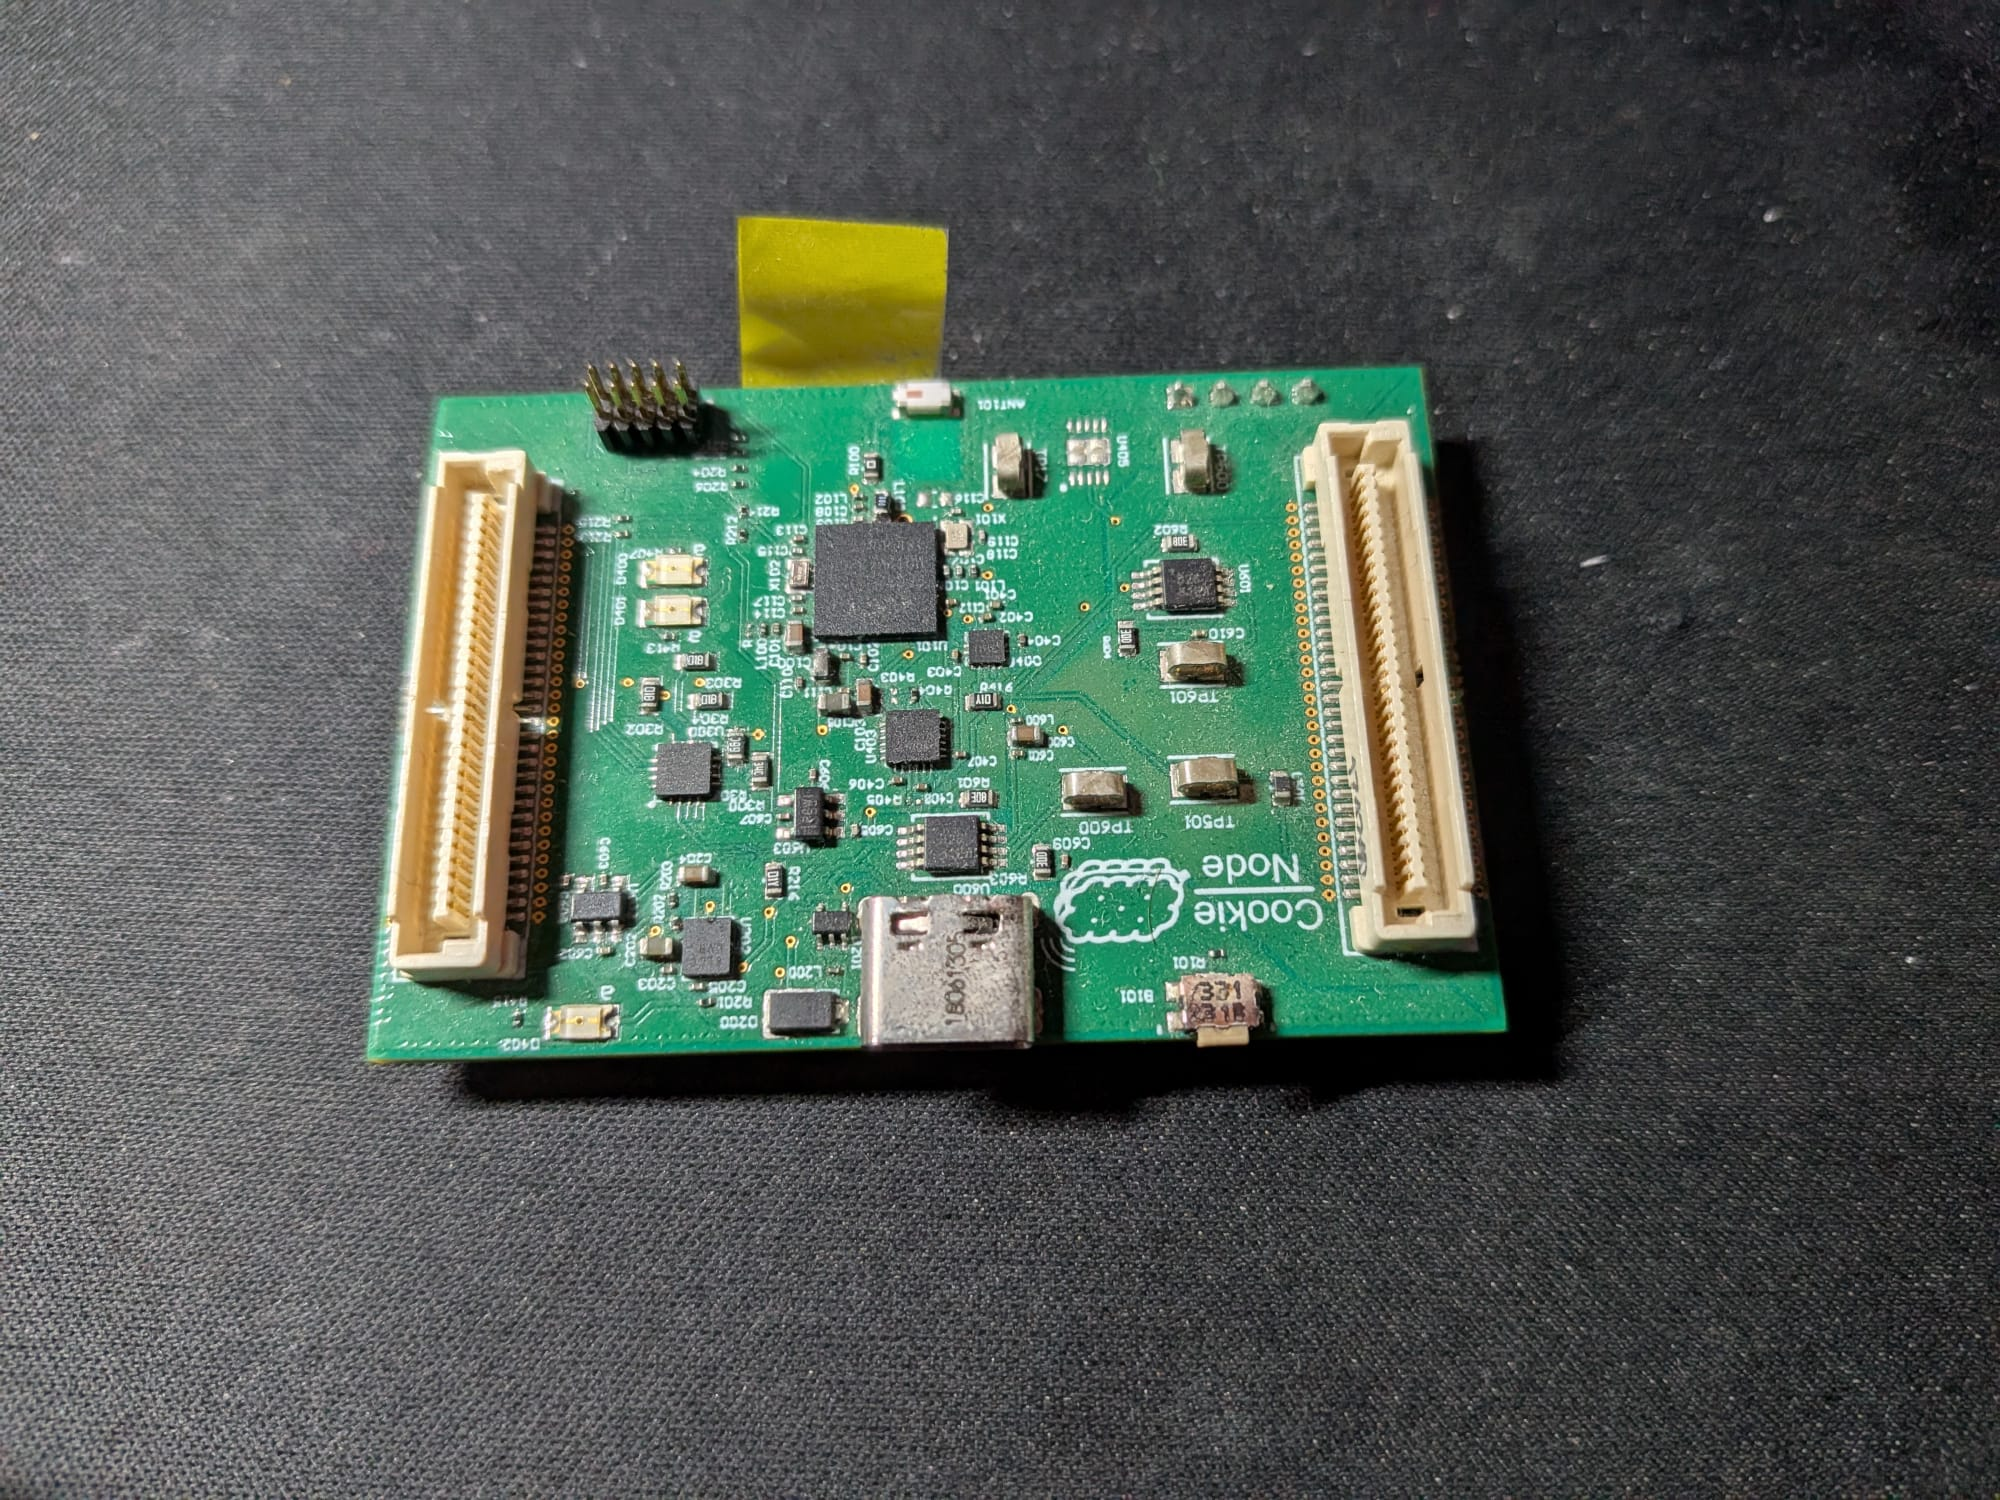
\includegraphics[width=\textwidth]{figures/COOKIE.jpeg}
        \caption*{(a) Nodo embebido Cookie.} % El asterisco evita que LaTeX le sume un número de figura independiente
        \label{fig:cookie}
    \end{minipage}
    \hfill
    % Subfigura (b)
    \begin{minipage}[b]{0.7\textwidth}
        \centering
        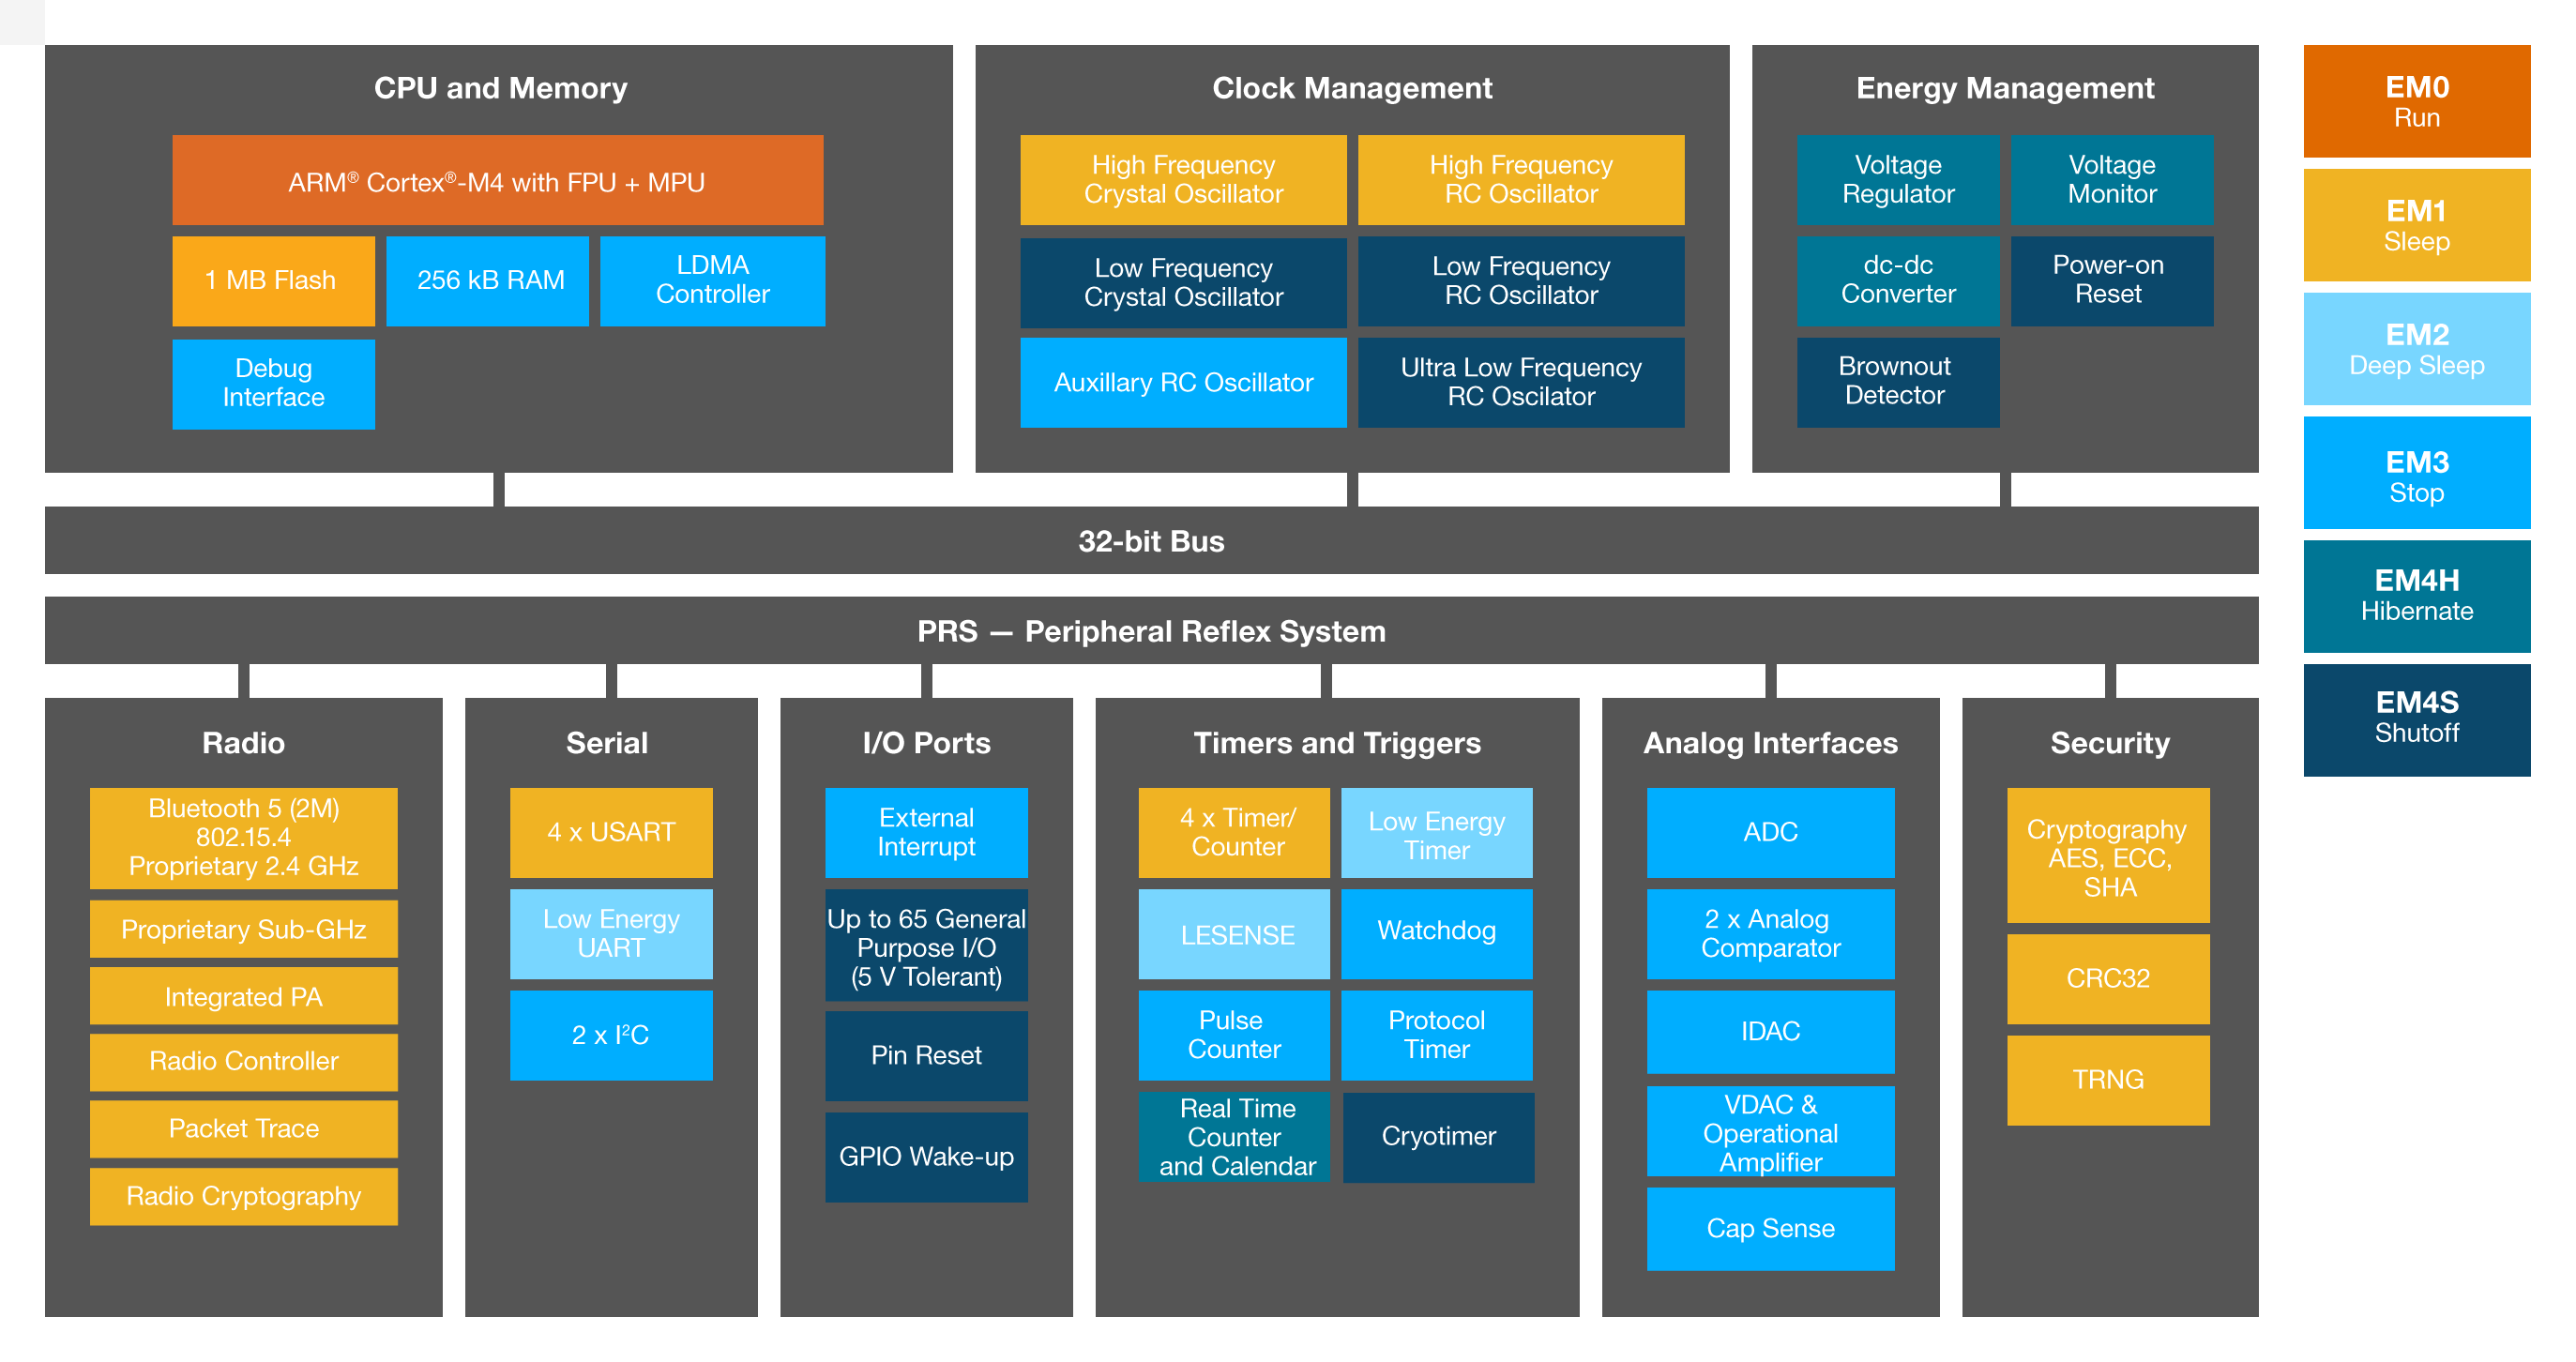
\includegraphics[width=\textwidth]{figures/EFR32.png}
        \caption*{(b) Diagrama de bloques funcional del SoC inalámbrico EFR32MG21.}
        \label{fig:efr32}
    \end{minipage}
    
    \vspace{0.3cm}
    % Título principal de la figura completa
    \caption{Componentes de hardware utilizados en el proyecto.}
    \label{fig:componentes_hardware}
\end{figure}


El núcleo ARM Cortex-M4, es una arquitectura ampliamente utilizada en sistemas embebidos, debido a que ofrece un gran equilibrio entre rendimiento 
y consumo de energia. Las características principales de este microcontrolador resultan relevantes, ya que las operaciones criptográficas deben ejecutarse sobre el nodo,
compartiendo los recursos disponibles como la pila de comunicaciones, el sistema de adquisición de datos y el resto de funcionalidades. El SoC integra una memoria Flash 
de hasta 1MB y 256 KB de memoria RAM. El SoC cuenta con un módulo RF integrado y configurable para las comunicaciones inalámbricas. Dependiendo de la variante, permite operar tanto en la banda
ISM de 2.4 GHz como en la banda Sub-GHz. Las comunicaciones empleadas en este trabajo se realizan en la banda de 2.4 GHz.

Por otro lado, el nodo embebido cuenta con un sensor de temperatura y humedad frabicado por Silicon Labs, \textit{Si7021} \cite{Si7021}, que permite la adquisición de datos ambientales. 
El sensor incorpora un convertidor analógico-digital, que permite una comunicación mediante una interfaz I2C. El sensor cuenta con un calibrado de fábrica y presenta una precisión 
máxiama de $\pm 3 \% RH$ para humedad relativa y $\pm 0,4 ªC$ para temperatura.

En la plataforma experimental, las medidas obtenidas por el sensor Si7021 se utilizan para genera un trafico de datos periodicos en la red empleada en el experimento.
De esta forma, el envio de temperatura y humedad constituye un flujo de datos que permite evaluar el rendimiento de la red. 

\section{Arquitectura del sistema} % Integracion de HQC en la plataforma Y Topologias de red 

Una vez presentada la plataforma experimental, se describe la arquitectura general del sistema. Esta se compone por dos tipos de nodos: cliente y servidor. Los nodos clientes 
se encargan de adquirir los datos ambientales y transmitirlos al servidor. Por otro lado, el nodo servidor se encarga de recibir y almacenar la información, asi como de 
gestionar las sesiones asociadas a cada nodo, coordinar el inicio y finalización de las pruebas y enviar instrucciones necesarias a los clientes. 

\begin{figure}[htbp]
    
    \centering
    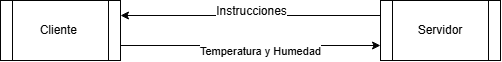
\includegraphics[width=0.8\textwidth]{figures/Arquitectura_C_S.png}
    \caption{Arquitectura general del sistema.} 

\end{figure}

En la Figura 3.3a se muestra el flujo principal de HQC del servidor, en cuanto el nodo servidor se inicia, genera el par de claves pública y privada, y queda a la 
espera de la llegada de un mensaje de inicio de sesión por parte del cliente, este mensaje se conoce como \textit{GETPK}. Una vez recibido,
el servidor responde con la clave pública. Cuando el servidor recibe el \(CT\), ejecuta el proceso de desencapsulación utilizando su clave privada y obtiene el mismo secreto compartido \(SS\) que se genero en el cliente. A partir de este momento, la sesión queda establecida 
y el servidor queda a la espera de la llegada de los datos cifrados del cliente. 

\begin{figure}[H]
    \centering
    % Subfigura (a)
    \begin{minipage}[b]{0.45\textwidth}
        \centering
        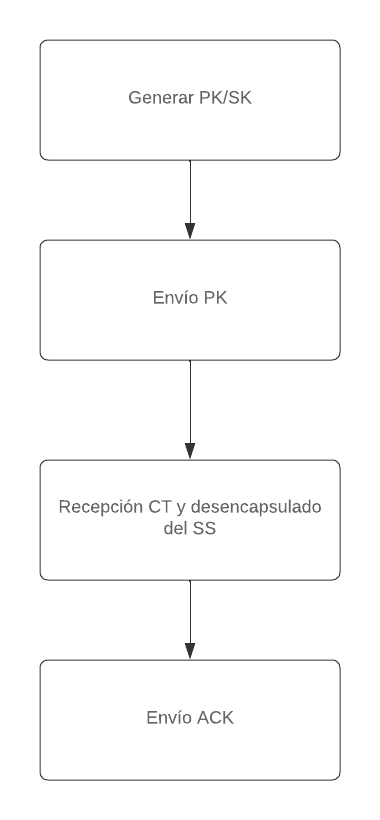
\includegraphics[width=0.6\textwidth]{figures/Arq_S.png}
        \caption*{(a) Arquitectura del servidor.} % El asterisco evita que LaTeX le sume un número de figura independiente
        \label{fig:ARQS}
    \end{minipage}
    \hfill
    % Subfigura (b)
    \begin{minipage}[b]{0.45\textwidth}
        \centering
        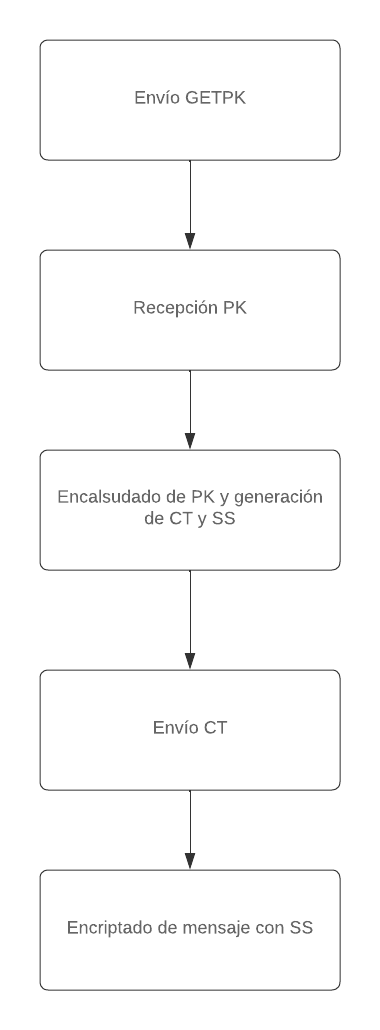
\includegraphics[width=0.6\textwidth]{figures/Arq_C.png}
        \caption*{(b) Arquitectura del cliente.}
        \label{fig:ARQC}
    \end{minipage}
    
    \vspace{0.3cm}
    % Título principal de la figura completa
    \caption{Arquitectura del sistema.}
    \label{fig:componentes_hardware}
\end{figure}

Por el lado del cliente, como se muestra en la Figura 3.3b, el flujo de HQC comienza con el envío del mensaje \textit{GETPK} al servidor.
Una vez recibida la clave pública del servidor, el cliente ejecuta el proceso de encapsulación utilizando dicha clave, obteniendo como resultado el texto cifrado \(CT\) y el secreto compartido \(SS\). Una vez que el cliente recibe la confirmacón
de que el servidor ha desencapsulado el CT correctamente, el cliente procede a cifrar los datos obtenidos del sensor y enviarlos al servidor. Una vez establecido el secreto compartido entre el cliente y el servidor, este se asocia a la sesíon del cliente, y es utilizado para proteger las posteriores comunicaciones de la aplicación.

La comunicación entre el cliente y el servidor sobre la pila de red proporcionada por Contiki-NG. Los mensajes son transportados mediante el protocolo UDP sobre IPv6, 
empleando 6LowPAN para su adaptación al enlace inalámbrico y RPL para establecer las rutas entre los distintos nodos de la red. 

La arquitectura descrita en este apartado se mantiene para las diferentes topologías de red implementadas durante los experimentos. Se implementaron cuatro topologías diferentes, 
estrella, linea, árbol y P2P, modificando el número de nodos y saltos existentes entre los clientes y el servidor. En la Figura 3.4 se muestran las topologías implementadas. 

\begin{figure}[htbp]
  \centering
  \begin{minipage}{0.9\textwidth} % Ancho del bloque completo
    \centering
    
    % --- FILA 1 ---
    \begin{minipage}{0.47\textwidth}
      \centering
      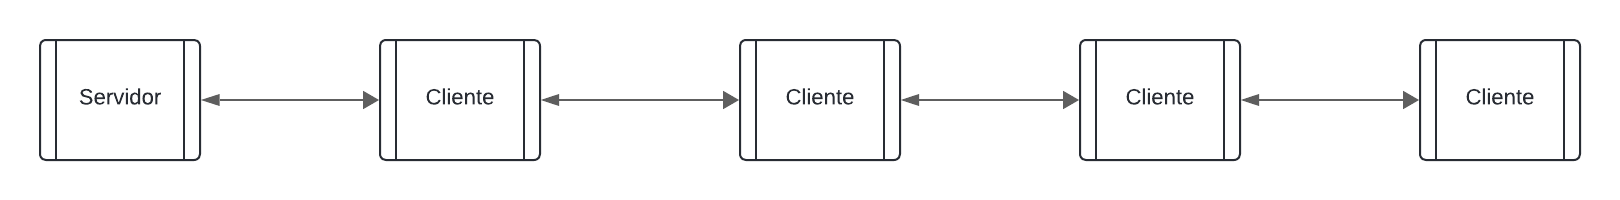
\includegraphics[width=\textwidth]{figures/Linea.png}
      \caption*{(a) Línea} % Si usas el paquete caption
      % Alternativa sin paquetes: \small (a) Línea
    \end{minipage}
    \hfill % Empuja la segunda imagen a la derecha
    \begin{minipage}{0.47\textwidth}
      \centering
      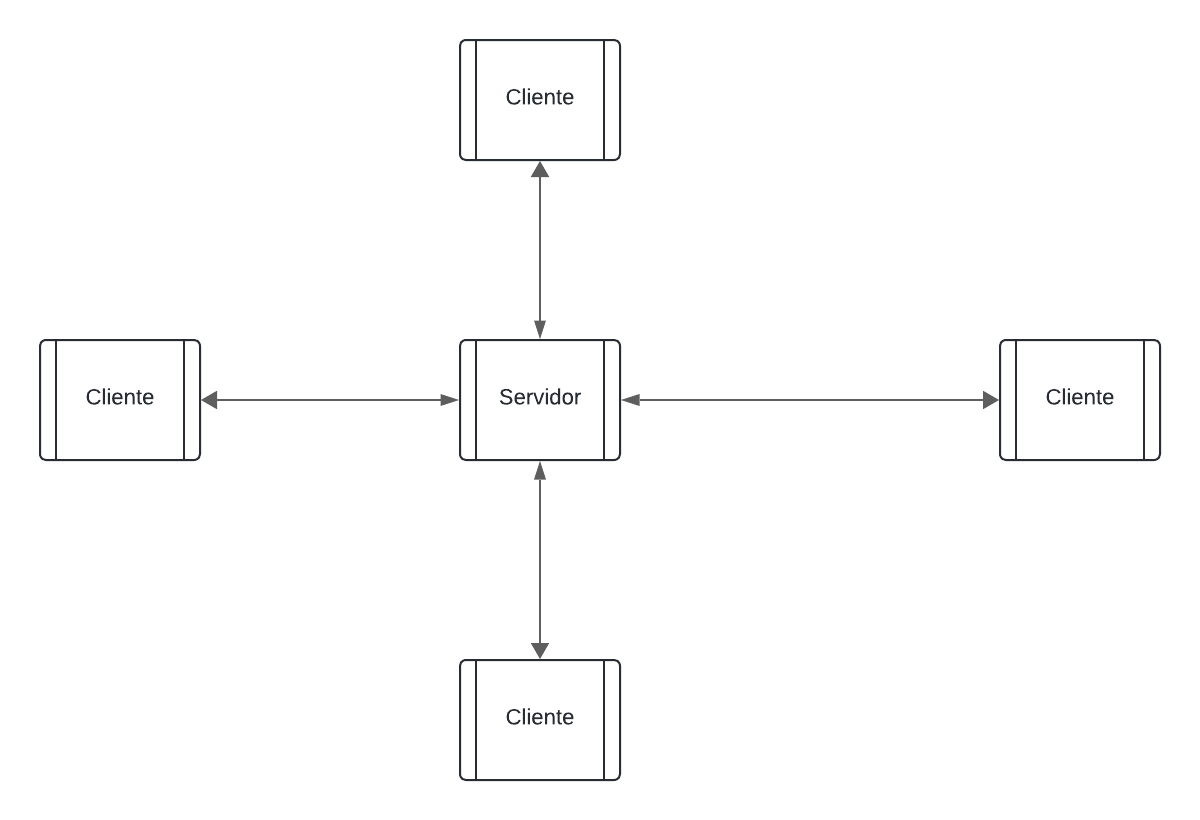
\includegraphics[width=\textwidth]{figures/Estrella.png}
      \caption*{(b) Estrella}
    \end{minipage}
    
    \vspace{0.6cm} % Separación vertical entre filas (un poco mayor para el texto)
    
    % --- FILA 2 ---
    \begin{minipage}{0.47\textwidth}
      \centering
      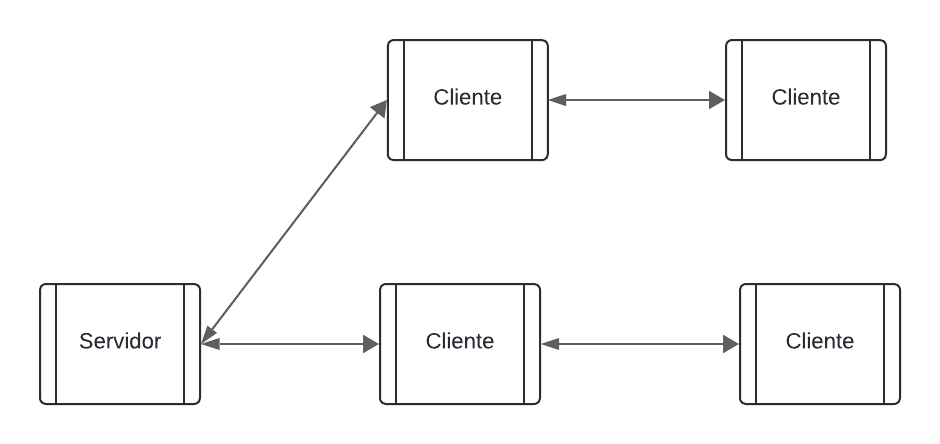
\includegraphics[width=\textwidth]{figures/arbol.png}
      \caption*{(c) Árbol}
    \end{minipage}
    \hfill
    \begin{minipage}{0.47\textwidth}
      \centering
      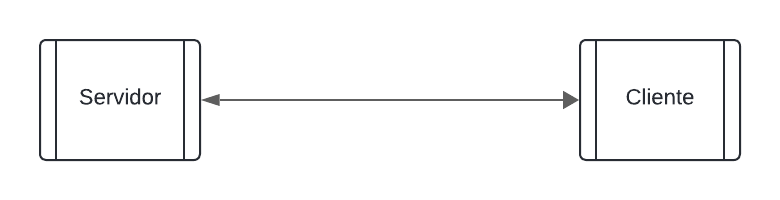
\includegraphics[width=\textwidth]{figures/P2P.png}
      \caption*{(d) P2P}
    \end{minipage}
    
    \vspace{0.3cm}
    \caption{Topologías implementadas.}
    \label{fig:cuadrandícula}
  \end{minipage}
\end{figure}


\section{Protocolo de intercambio y transporte de HQC}


\section{Sistema de adquisición de métricas}

\section{Corrección del subsistema de comunicaciones}
\subsection{Sintomas iniciales}
\subsection{Proceso de diagnostico}
\subsection{Modificacion del driver}
\subsection{impacto sobre el trabajo}
